%%%%%%%%%%%%%%%%%%%%%%%%%%%%%%%%%%%%% BEGIN HEADERS %%%%%%%%%%%%%%%%%%%%%%%%%%%%%%%%%%%%%%%%%%%%%%%%%%%%%
\documentclass[11pt,conference]{IEEEtran}

\usepackage{longtable}
\usepackage{graphicx}
\usepackage[utf8]{inputenc}
\usepackage{fancyhdr}
\usepackage{float}
\usepackage[hidelinks]{hyperref}
\usepackage{listings}
\usepackage{color}
\usepackage{natbib}
\usepackage{amsmath}

% Your names in the header
\pagestyle{fancy}
\rhead{Enrico Tedeschi}
\lhead{INF-3201 Parallel Programming - Assignment 2}
\cfoot{\thepage}

% Used for including code in a stylized manner
\definecolor{codegreen}{rgb}{0,0.6,0}
\definecolor{codegray}{rgb}{0.5,0.5,0.5}
\definecolor{codepurple}{rgb}{0.58,0,0.82}
\definecolor{backcolour}{rgb}{0.95,0.95,0.92}
 

\lstdefinestyle{mystyle}{
    backgroundcolor=\color{backcolour},   
    commentstyle=\color{codegreen},
    keywordstyle=\color{magenta},
    numberstyle=\tiny\color{codegray},
    stringstyle=\color{codepurple},
    basicstyle=\footnotesize,
    breakatwhitespace=false,         
    breaklines=true,                 
    captionpos=b,                    
    keepspaces=true,                 
    numbers=left,                    
    numbersep=5pt,                  
    showspaces=false,                
    showstringspaces=false,
    showtabs=false,                  
    tabsize=2
}

\lstset{style=mystyle}

% The Title
\title{INF-3201 Parallel Programming
\newline
Shared Memory}

% Your name and email
\author{\textbf{Enrico Tedeschi}\\ ete011@post.uit.no }


%%%%%%%%%%%%%%%%%%%%%%%%%%%%%%%%%%%%% END HEADERS %%%%%%%%%%%%%%%%%%%%%%%%%%%%%%%%%%%%%%%%%%%%%%%%%%%%%

\begin{document}

% Create the title and everything
\maketitle

\section{Introduction}
The goal of this assignment is to parallelize a piece of code using shared memory techniques preferably using \textbf{OpenMP}.
\newline
The piece of code to parallelize could be the given one, that is a Markovian chess engine, or a chosen piece of code which has to be approved by the professor.
\subsection{Requirements}
\begin{itemize} 
\item Choose a piece of software to parallelize
\item Parallelize it with shared-memory techniques
\item Evaluate speedup
\end{itemize}

\section{Technical Background}

\begin{itemize} 
\item[--] Concurrency and parallelism concepts
\item[--] Parallel programming concepts
\item[--] Basic programming approach
\item[--] Knowledge of C language
\item[--] Notion of design pattern principles
\item[--] Theory about software engineering
\item[--] Knowledge of git to manage the software versions
\end{itemize}


\section{Analysis}
The given \textbf{Markovian} code was found to be too long and quite hard to understand, in addition, it has no deterministic solution so it would have been really difficult to test.
\newline
The code chosen to be parallelized is a sequential version of the \textbf{TSP} (Traveller Salesman Problem). It asks the following question: \textit{Given a list of cities and the distances between each pair of cities, what is the shortest possible route that visits each city exactly once and returns to the origin city?} \cite{citation1}
\newline
The sequential code was refined by adding a random function which generates distances between cities and also the possibility of running the programme with a size passed as a parameter was implemented.
\newline
To parallelize a sequential code is necessary to analyse which function involves the biggest amount of time. The given program, \textit{tsp-seq.c}, has been tested with \textit{profile} and the following table is the result of this test:
\begin{lstlisting}
  %   cumulative   self               
 time   seconds    calls   name    
100.32   2.90        1     zRoute
  0.00   0.00      196     zEuclidDist
  0.00   0.00       28     random_at_most
  0.00   0.00        2     second
  0.00   0.00        1     zReadRoute
\end{lstlisting}

Looking at this table it turns out that the function to parallelize is obviously \textit{zRoute}.
\newline
The function has a recursive structure for each possible successor of the city chosen as initial. For instance, if the function would have a $iSize = 5$ (number of cities) then the execution tree would look like the one in Fig \ref{fig:tree}. 
In the first 'level' of the tree the first city executes recursively the $zRoute$ function for the number of the cities left to visit, and so for the other levels.
Having an image of the execution tree helps to get the parallelization easier.
\begin{figure}[h!]
  \centering
    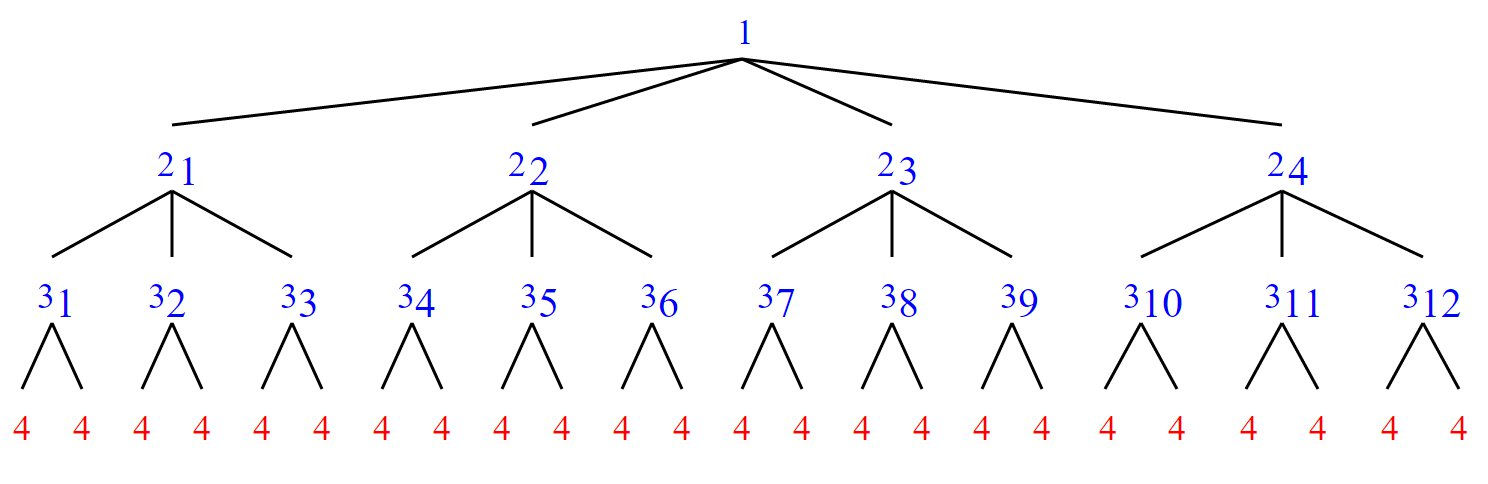
\includegraphics[width=0.5\textwidth]{tree}
    \caption{Execution of the zRoute function}
    \label{fig:tree}
\end{figure}
\newline
The sequential version has a time of execution which is terribly exponential, changing between 16 and 17 cities involves a time of execution from 40 to 190 seconds. The "superexponential" graph is represented in Fig \ref{fig:node-scaling-seq}.
That is why the tsp is a perfect problem to parallelize.
\begin{figure}[h!]
  \centering
    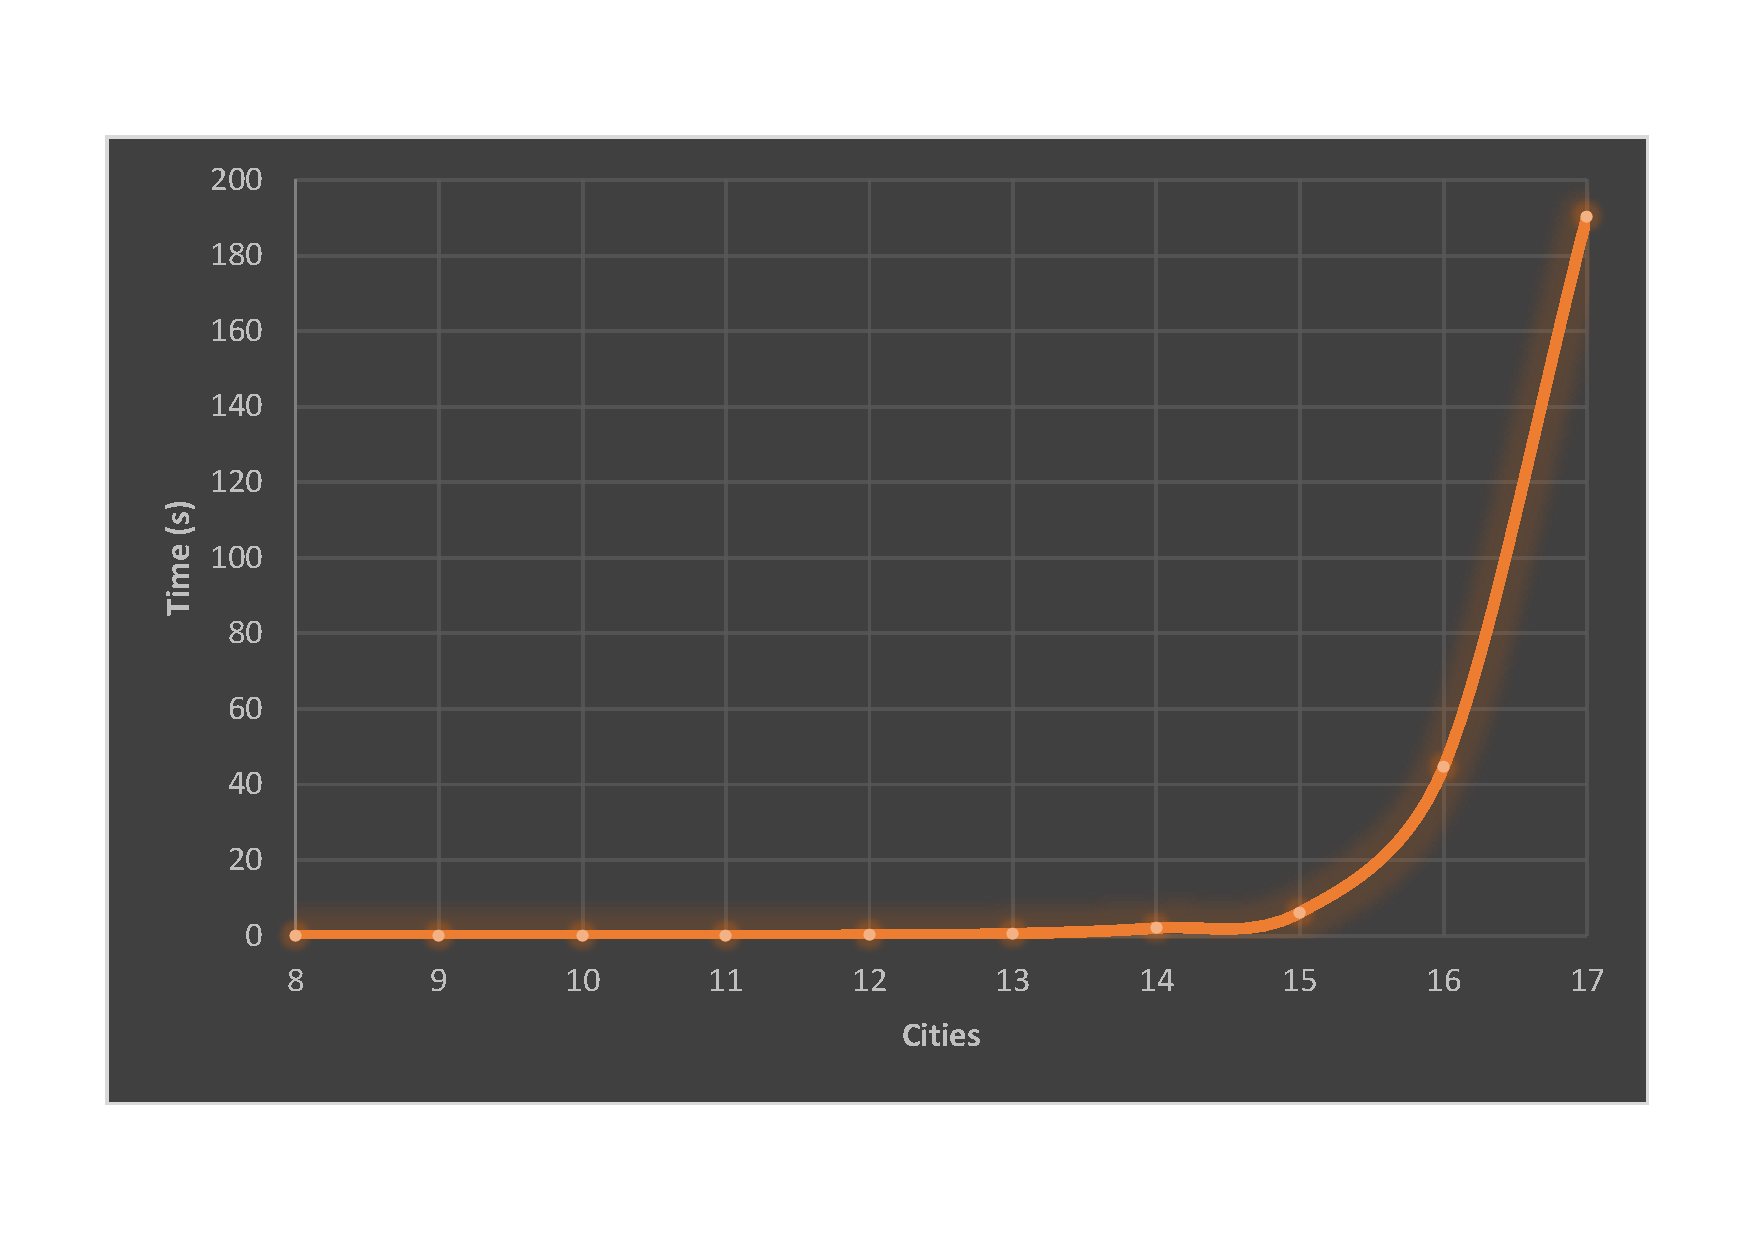
\includegraphics[trim=0.0cm 3.5cm 0.0cm 3.5cm, width=0.5\textwidth]{node-scaling-seq}
    \caption{Execution time of the sequential version of tsp}
    \label{fig:node-scaling-seq}
\end{figure}
\section{Implementation}
\subsection{Environment}
The code has been developed using JetBrains CLion 1.1 on Windows 10 and due to a more easy way to compile and test the MPI programs with a Linux based console, the compilation and the execution of the code has been made on an Ubuntu Virtual Machine with 4 core assigned, using VirtualBox 4.2 and Ubuntu version 14.04.3
\newline
To synchronize the cluster and the local machine and to keep trace of all the changes in the code, a git repository was created and the git command on linux were used to commit and to push/pull data from repositories.
\newline
The benchmarking and the test with more than 4 cores has been done in the UiT uvrocks cluster. The connection with the cluster was established by using ssh on a linux machine:
\begin{lstlisting}
ssh -X -A ete011@uvrocks.cs.uit.no
\end{lstlisting}
To simplify the execution of the code, a proper Makefile was implemented.

\subsection{Fixing the Sequential Version}
Before starting the parallelization some changes to the sequential version were implemented. The way to verify if the solution found is reliable is to check the $length$ of the path to visit all the cities. The length of the path changes if either the number of the cities, the size of the map or where the cities are located is changed. Considering that, the function \textit{random\_at\_most(max\_size)} is implemented. It generates the same random numbers given a certain input from \textit{0 to max\_size} in this way is possible to test the \textit{crc} in a correct way without inserting the coordinates every time or without having duplicate or long and useless code.
The sequential version, \textit{tsp-seq.c}, takes as input the number of cities and it has a fixed map size.

\subsection{Approaching the Problem}
Due to the tricky recursive function the first goal of the implemented parallelization was: "get the speedup keeping the code simple". 
The Fig \ref{fig:tree-par} shows the logic used for the parallelization. The parts of the tree enhanced in red are the component which will run in parallel; in that way the speedup is strongly dependent from the relation between the $number\_of\_cores$ and the $number\_of\_cities$. Using this kind of approach the parallelization is made in the first $for$ cycle, and each core will execute the recursive function, solving all the sub-branches problems related to it.

\begin{figure}[h!]
  \centering
    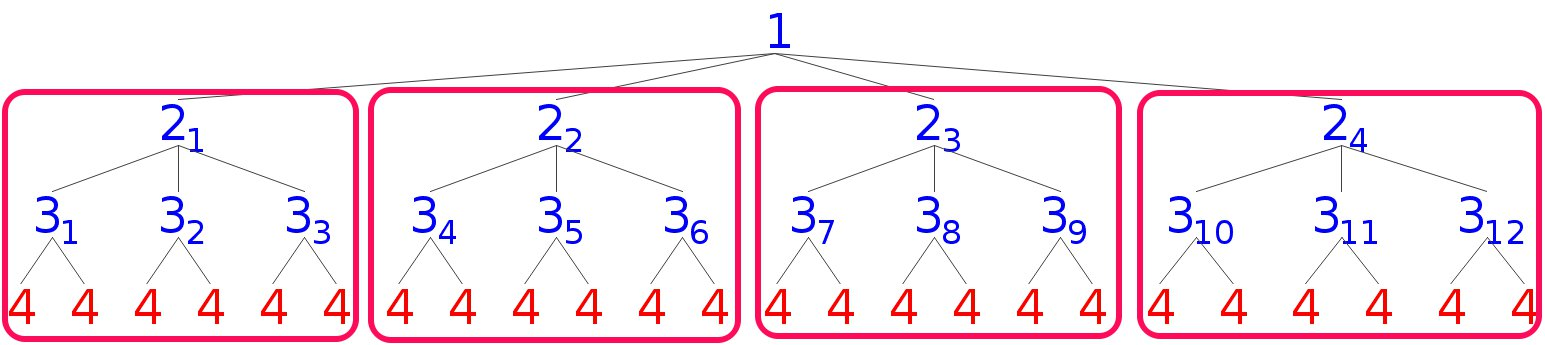
\includegraphics[width=0.5\textwidth]{tree-par}
    \caption{Execution of the parallel version of the zRoute function, with 5 cities using 4 parallel cores}
    \label{fig:tree-par}
\end{figure}

\subsection{Parallelization}
For the parallelization \textbf{OpenMP} API were used. They provide to standardize directive-based multi-language high-level parallelism that is performant, productive and portable\cite{citation4}. Since the $zRoute$ function is recursive is necessary to define two types of $zRoute$ functions, a \textbf{sequential} one and a \textbf{parallel} one. If the code is in the first level of the tree, then it will call for each sub-branches the recursive parallel function, otherwise it will call the sequential one.
\newline
The biggest problem to solve was related to shared memory and how the variables were used while parallelizing the code. OpenMp indeed takes care about the balancing of the work but is necessary to have well defined which variable needs to be global and which ones local.
\newline
To parallelize the function the following logic was used:
\begin{lstlisting}
count = 0;
void zRoute(...){
    if (count == 0) {
    	count++;
    	#pragma omp parallel num_threads(#)
    	{
    	#pragma omp for
    	--core of zRoute function--
    	}
    }
    else{
    	--core of zRoute function--
    }
    return;
}
\end{lstlisting}

To keep the variables local, a strong analysis on them has been done. All the variables which change their value during the execution (called $var\_c$ in the listing below) of zRoute must have been declared locally. To achieve that, a function called \textit{for\_cycle\_zRoute} has been created and it is called only when $count = 0$, that is  when the code needs to be parallelized. Therefore the function it receives as input all these variables which need to be locally declared and it executes the core of the zRute function.

\begin{lstlisting}
void zRoute(...){
    if (count == 0) {
    	#pragma omp parallel num_threads(#)
    	{
    		for_cycle_zRoute(var_c);
    	}
    }
    else{
    	--core of zRoute function--
    }
    return;
}
\end{lstlisting}

The logic for the \textit{for\_cycle\_zRoute} function is:

\begin{lstlisting}
void for_cycle_zRoute(var_c){
    --definition of local variables--
    #pragma omp for
    --core of zRoute function--
    return;
}
\end{lstlisting}
\section{Result and Benchmarking}
The sequential and the parallel programs were tested on uvrocks cluster. During the evaluation, the \textbf{speedup}, the \textbf{efficiency} and the scaling with the number of cities and cores were taken into consideration.
\newline

\subsection{Speedup}
\[ S(p) = \dfrac{t_s}{t_p}  \]
where $t_s$ is the sequential time and $t_p$ is the parallel time using p processors. As the Fig \ref{fig:speedup} shows, the speedup achieved is not strongly dependent from the number of cores used and doesn't matter how many cores will be used but the speedup will never be higher than 4x times the sequential one.

\begin{figure}[h!]
  \centering
    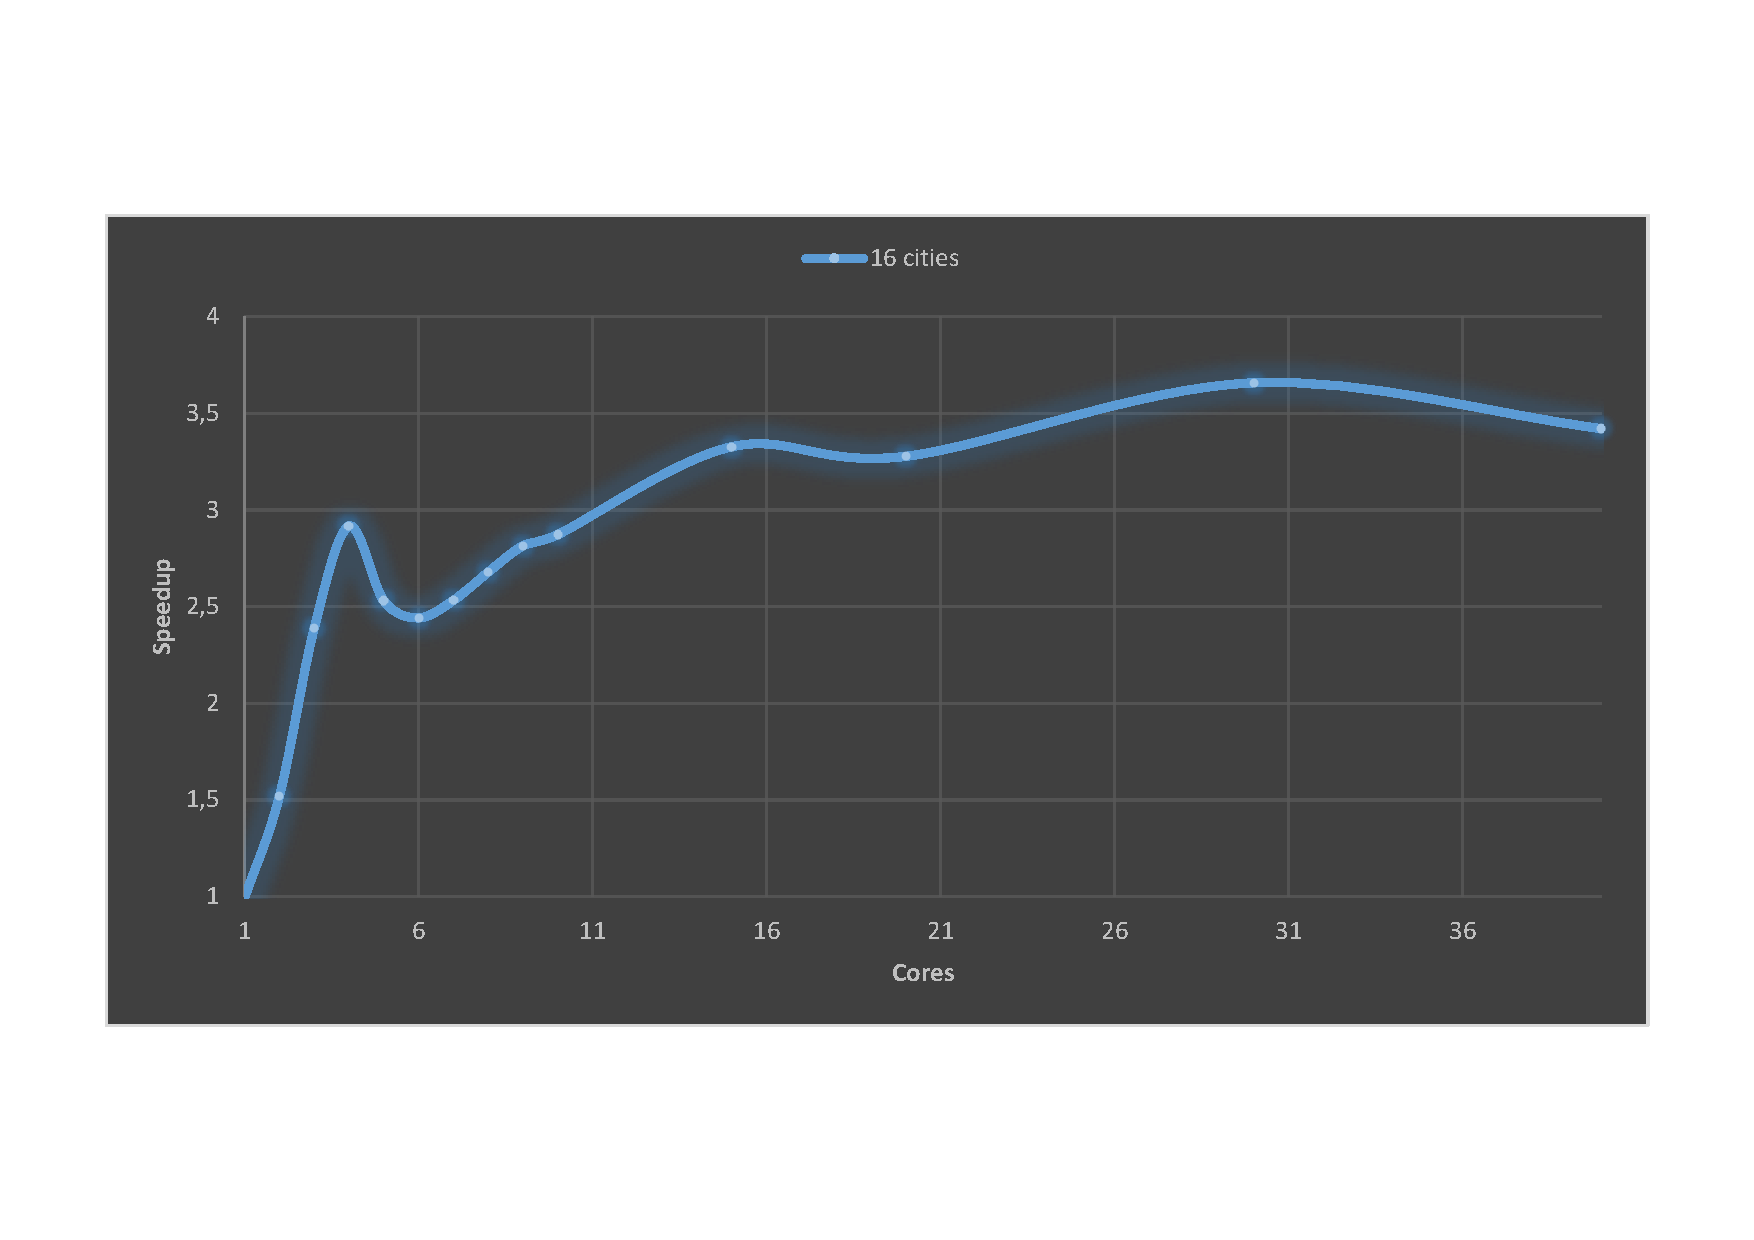
\includegraphics[trim=0.0cm 3.5cm 0.0cm 3.5cm, width=0.5\textwidth]{speedup}
    \caption{Speedup using 16 cities}
    \label{fig:speedup}
\end{figure}

This is due to the way of parallelizing the problem, it only splits the work at the first iteration, so even if there will be a lot of cores they will never be used anyway and in addition they will take extra time in the computation because of the message exchange for the communication between threads. This is confirmed in the evaluation of the efficiency, Fig \ref{fig:efficiency}.
 
\subsection{Efficiency}
\[ S(p) = \dfrac{t_s}{t_p * p}  \]
where p is the number of processes used. So the question which efficiency answers is: \textit{"How good is the parallelization using p number of cores?"}. The Fig \ref{fig:efficiency} represents the efficiency considering the executions from 1 to 40 cores, with number of cities equal to 16.

\begin{figure}[h!]
  \centering
    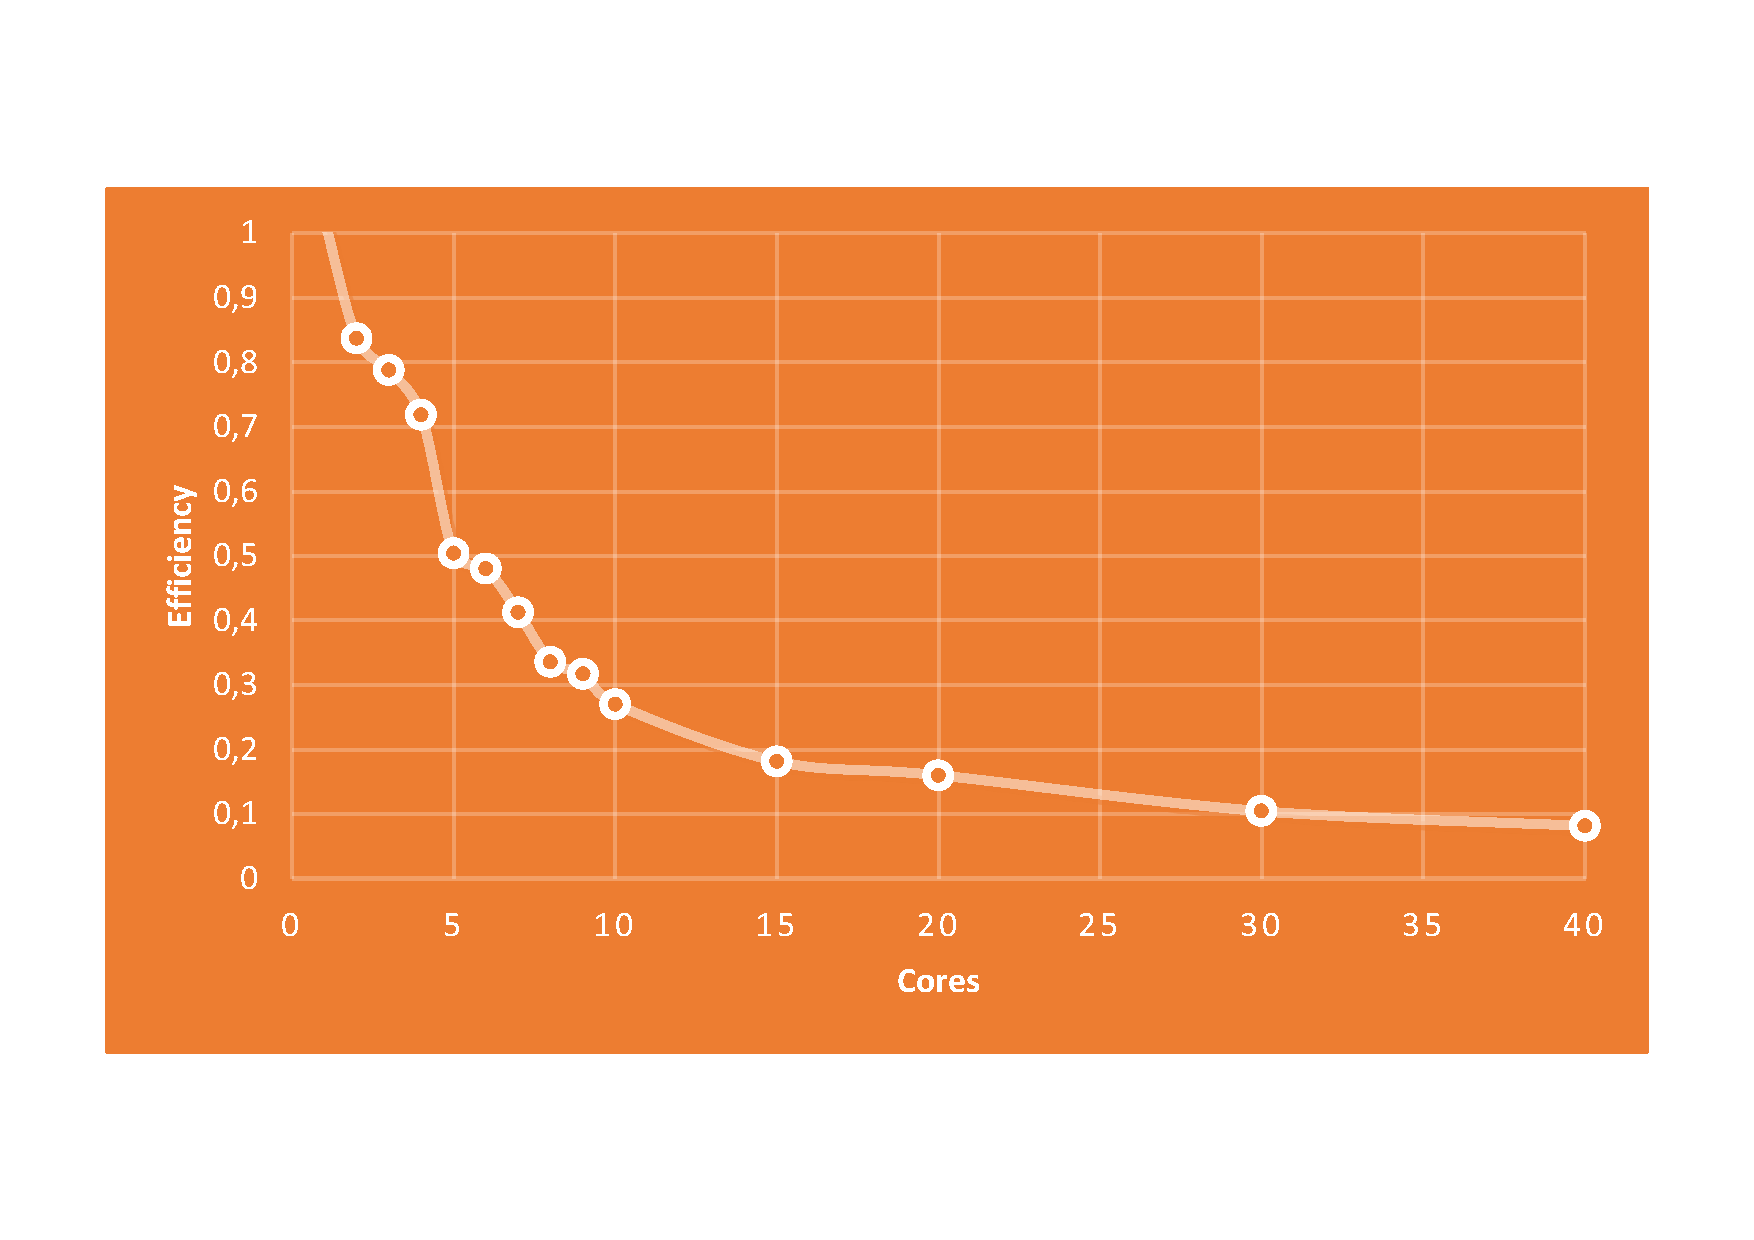
\includegraphics[trim=0.0cm 3.5cm 0.0cm 3.5cm, width=0.5\textwidth]{efficiency}
    \caption{Efficiency of the parallelization with 16 cities}
    \label{fig:efficiency}
\end{figure}

As said before, the efficiency is not good using more cores but it could be improved by letting the inactive processors to solve some sub-branches already ready to be solved.
\newline
The scaling of how the efficiency changes according to the number of city involved is not represented since it is the same for each number of city tested.

\begin{figure}[h!]
  \centering
    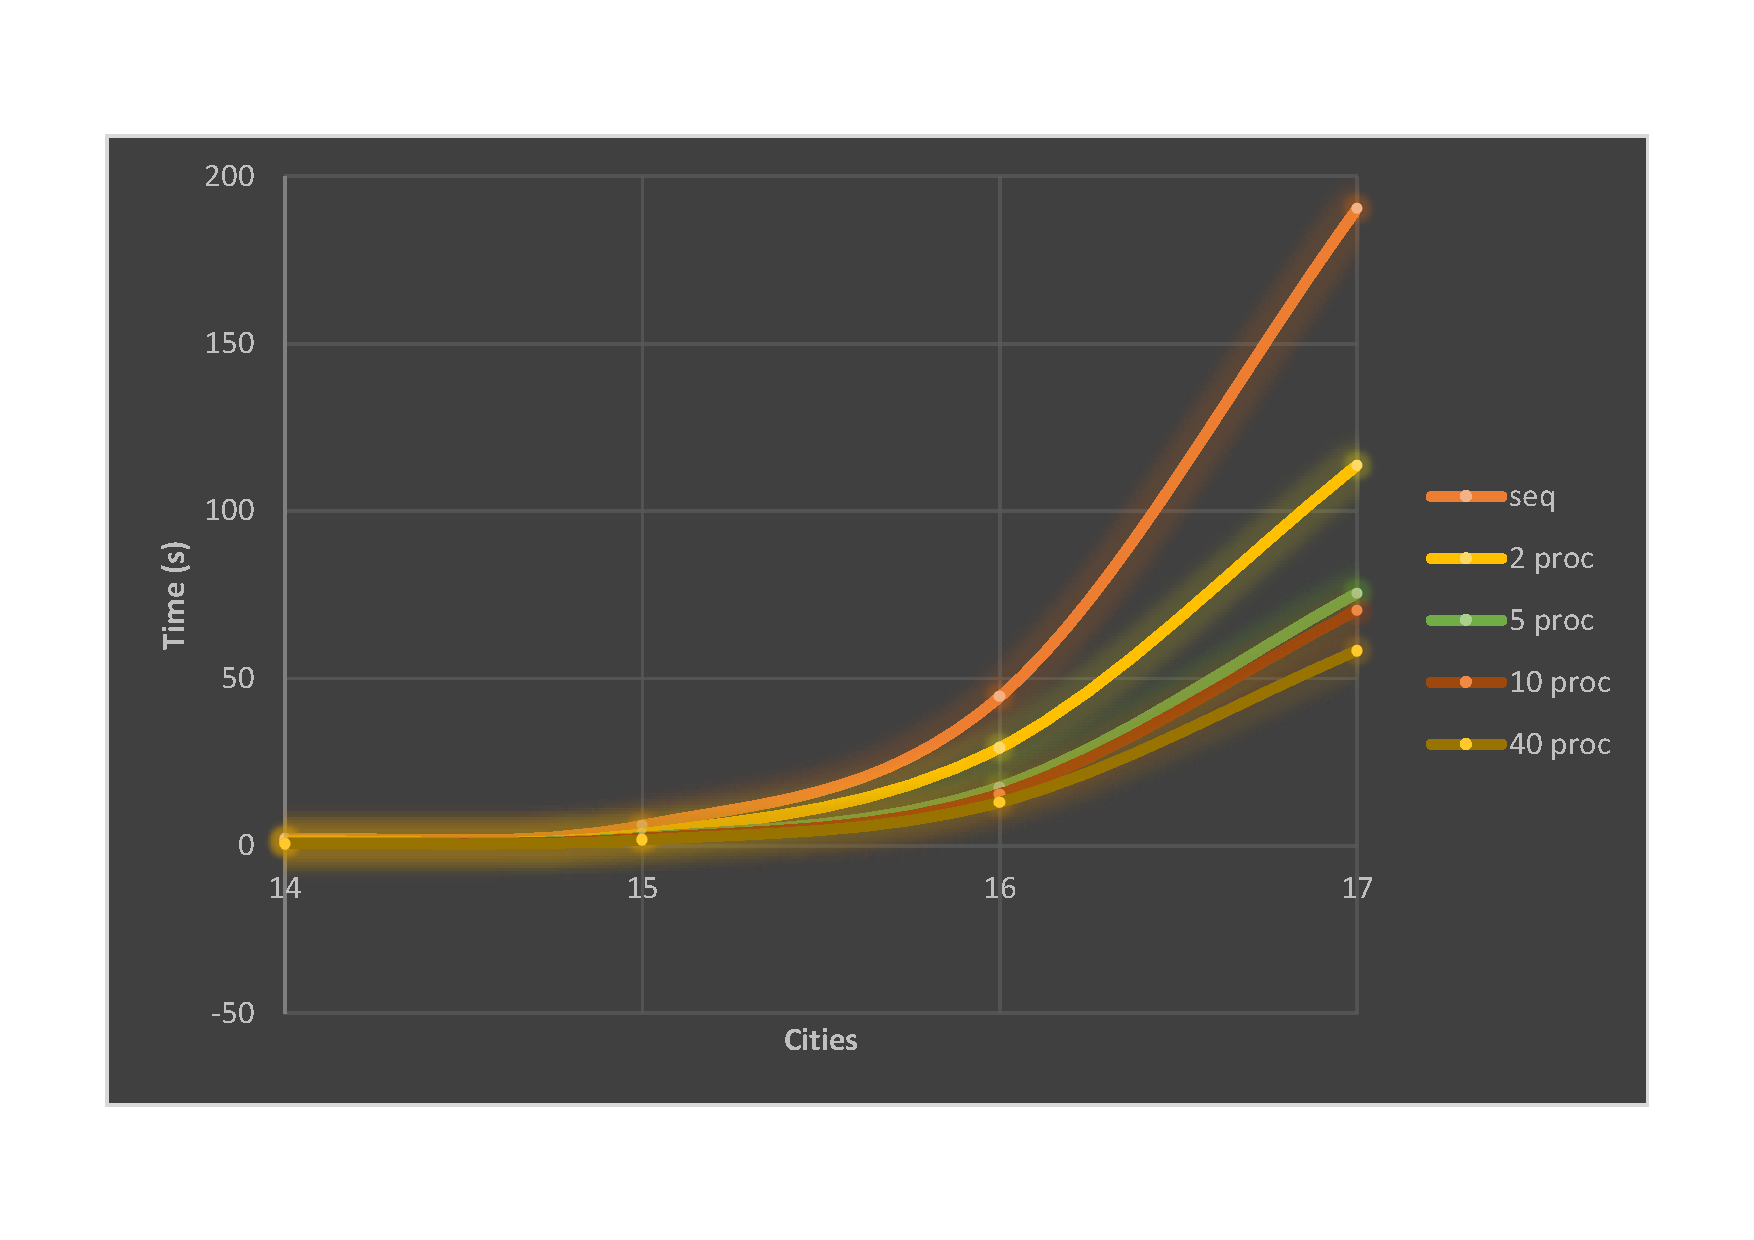
\includegraphics[width=0.5\textwidth]{time-comparsion}
    \caption{Execution time scaling the number of cities with different cores.}
    \label{fig:time-comparsion}
\end{figure}

\subsection{Scaling}
The scaling was implemented considering the number of cities and the threads used for the computation.
\newline
If the parallelization to the graph represented in Fig \ref{fig:node-scaling-seq} is applied, the improvement obtained is showed in Fig \ref{fig:time-comparsion}. The computation time is anyway "superexponential" but definitely faster than the sequential one, since the speedup obtained, as the Fig \ref{fig:speedup-comparsion} shows, it changes from 1x to 3.5x compared to the sequential one. Indeed the graph in Fig \ref{fig:speedup-comparsion} represents the speedup, scaling the number of cities and the cores. The cities taken into consideration change from a number of 8 to 17. Considering less than 8 cities the computation time would have been too low and not analysable and considering more than 17 cities the computation time would have been too high, only thinking that running 18 cities with 50 cores the computation time is 374 seconds and 369 second running 18 cities with 17 cores makes no sense in evaluating any further number of cities. The sequential time with 18 cities is 1358 seconds, which confirm the max 4x speedup gained.

\begin{figure}[h!]
  \centering
    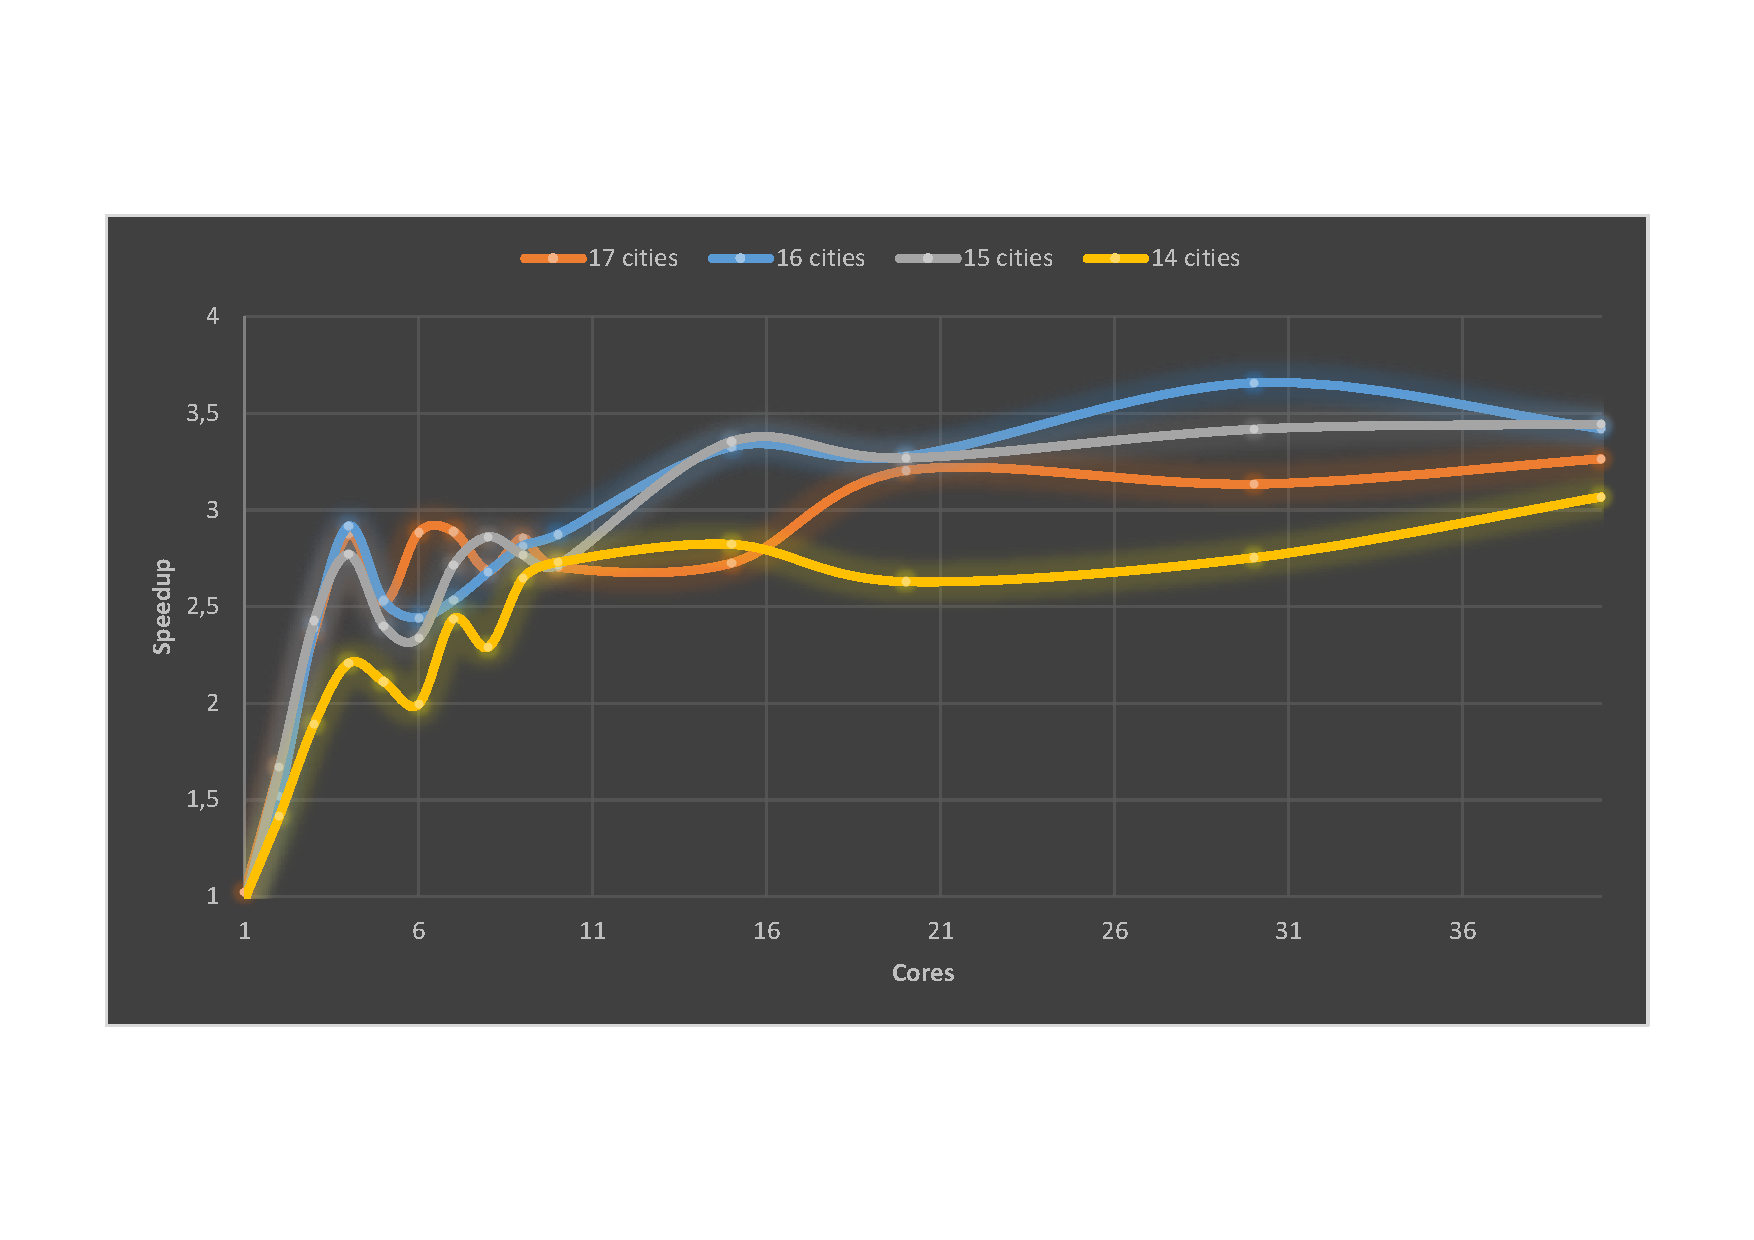
\includegraphics[width=0.5\textwidth]{speedup-comparsion}
    \caption{Speedup scaling the number of city involved.}
    \label{fig:speedup-comparsion}
\end{figure}

\section{Discussion}
Considering that even with the parallelization the execution time get a speedup only of 4x, is possible to improve it further. The main problem is that in this parallel version the workload is divided according of the number of $nodes - 1$; so if 5 cities are evaluated, 4 cores take the control of the four different branches, executing each branch in $(nodes - 1)!$ time. A possible optimization could involve the parallelization of each sub branches since the number of cities is known, is also known the total amount of sub problems to solve, in that way is possible to parallelize the work also for each sub problem if there is any free core waiting, like in the Fig \ref{fig:optimized-tree} where the blue enhanced parts indicate a further parallelization. It's possible to do that by creating a pull of work where each sub problem is stored and it gets deleted once done. It should be necessary, however, to synchronize the work done for each thread according to the part of the tree depth evaluated. This implementation is really fragile because, in case the next parallelized for loop requires 5 more cores to solve the sub problems but only 2 are available, then the whole "family" of problems which are related to the selected one will be waiting for the sub problems to get solved, generating in that way a huge waste of computation time. This could be avoided by keeping the two different implementation of the \textit{zRoute} function , and if there are not any processes available then execute the sequential version.
\newline
Implementing this, the problem of $n\_cores >> n\_cities$ is solved and it will be possible to get a better speedup.

\begin{figure}[h!]
  \centering
    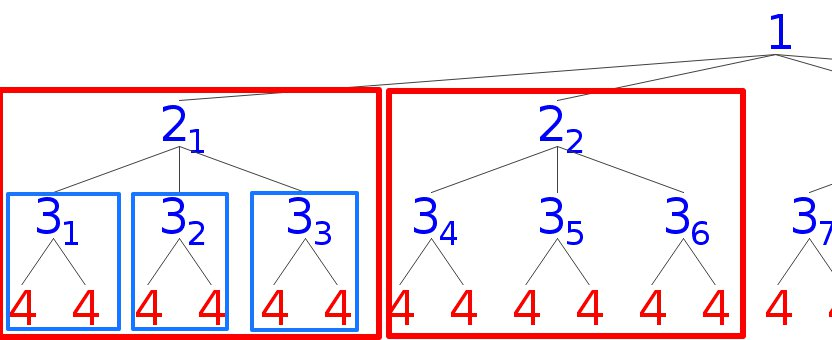
\includegraphics[width=0.5\textwidth]{optimized-tree}
    \caption{Possible implementation to further improve the parallelization.}
    \label{fig:optimized-tree}
\end{figure}

\section{Conclusion}
I can be satisfied even if the speedup is not the best I could have get because I had to work on this project in a really short time and the given code was barely readable so I spent quite few time trying to understand it properly.
In addition, parallelizing the recursive function was harder than expected ant it required plenty of time and a good analysis of the problem.
For this project I worked together with the colleague Gregor Decristoforo and the results obtained are pretty much the same.

\bibliographystyle{plain}
\bibliography{report}


\end{document}

